\item \points{25} {\bf A Simple Neural Network}

Let $X = \{x^{(1)}, \cdots, x^{(\nexp)}\}$ be a dataset of $\nexp$ samples with 2 features, i.e $\xsi \in \R^2$. The samples are classified into 2 categories with labels $\ysi \in \{0, 1\}$. A scatter plot of the dataset is shown in Figure $\ref{fig:nn_plot}$:
\begin{figure}[htbp]
    \centering
    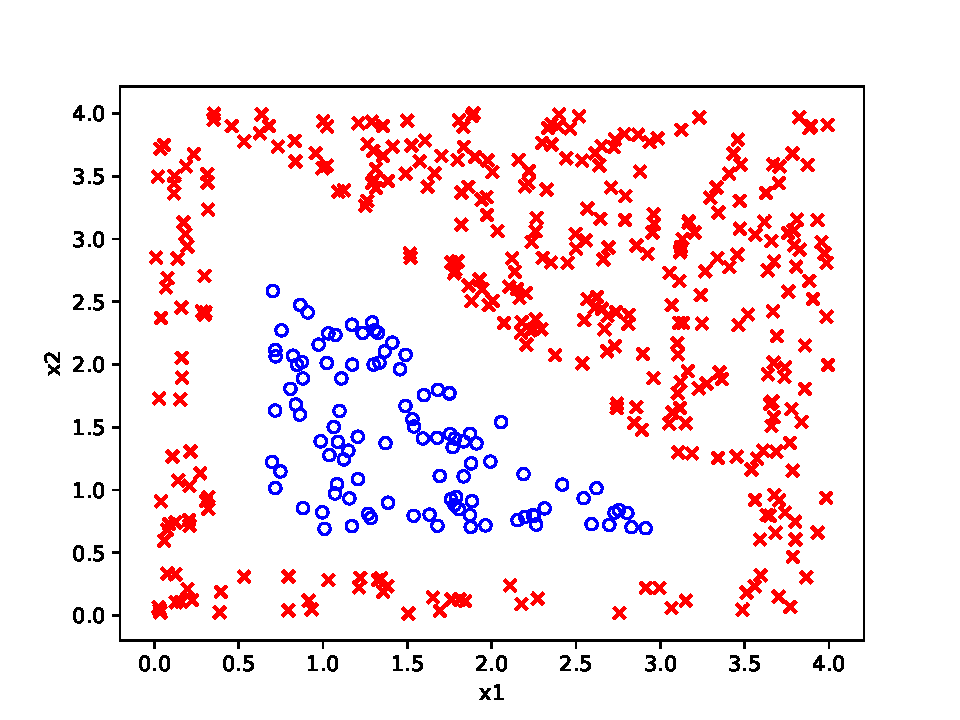
\includegraphics[scale=0.5]{simple_nn/nn_plot.pdf}
    \caption{Plot of dataset $X$.}
    \label{fig:nn_plot}
\end{figure}

The examples in class $1$ are marked as as ``$\times$" and examples in class $0$ are marked as ``$\circ$". We want to perform binary classification using a simple neural network with the architecture shown in Figure $\ref{fig:nn_arc}$:
\begin{figure}[htbp]
    \centering
    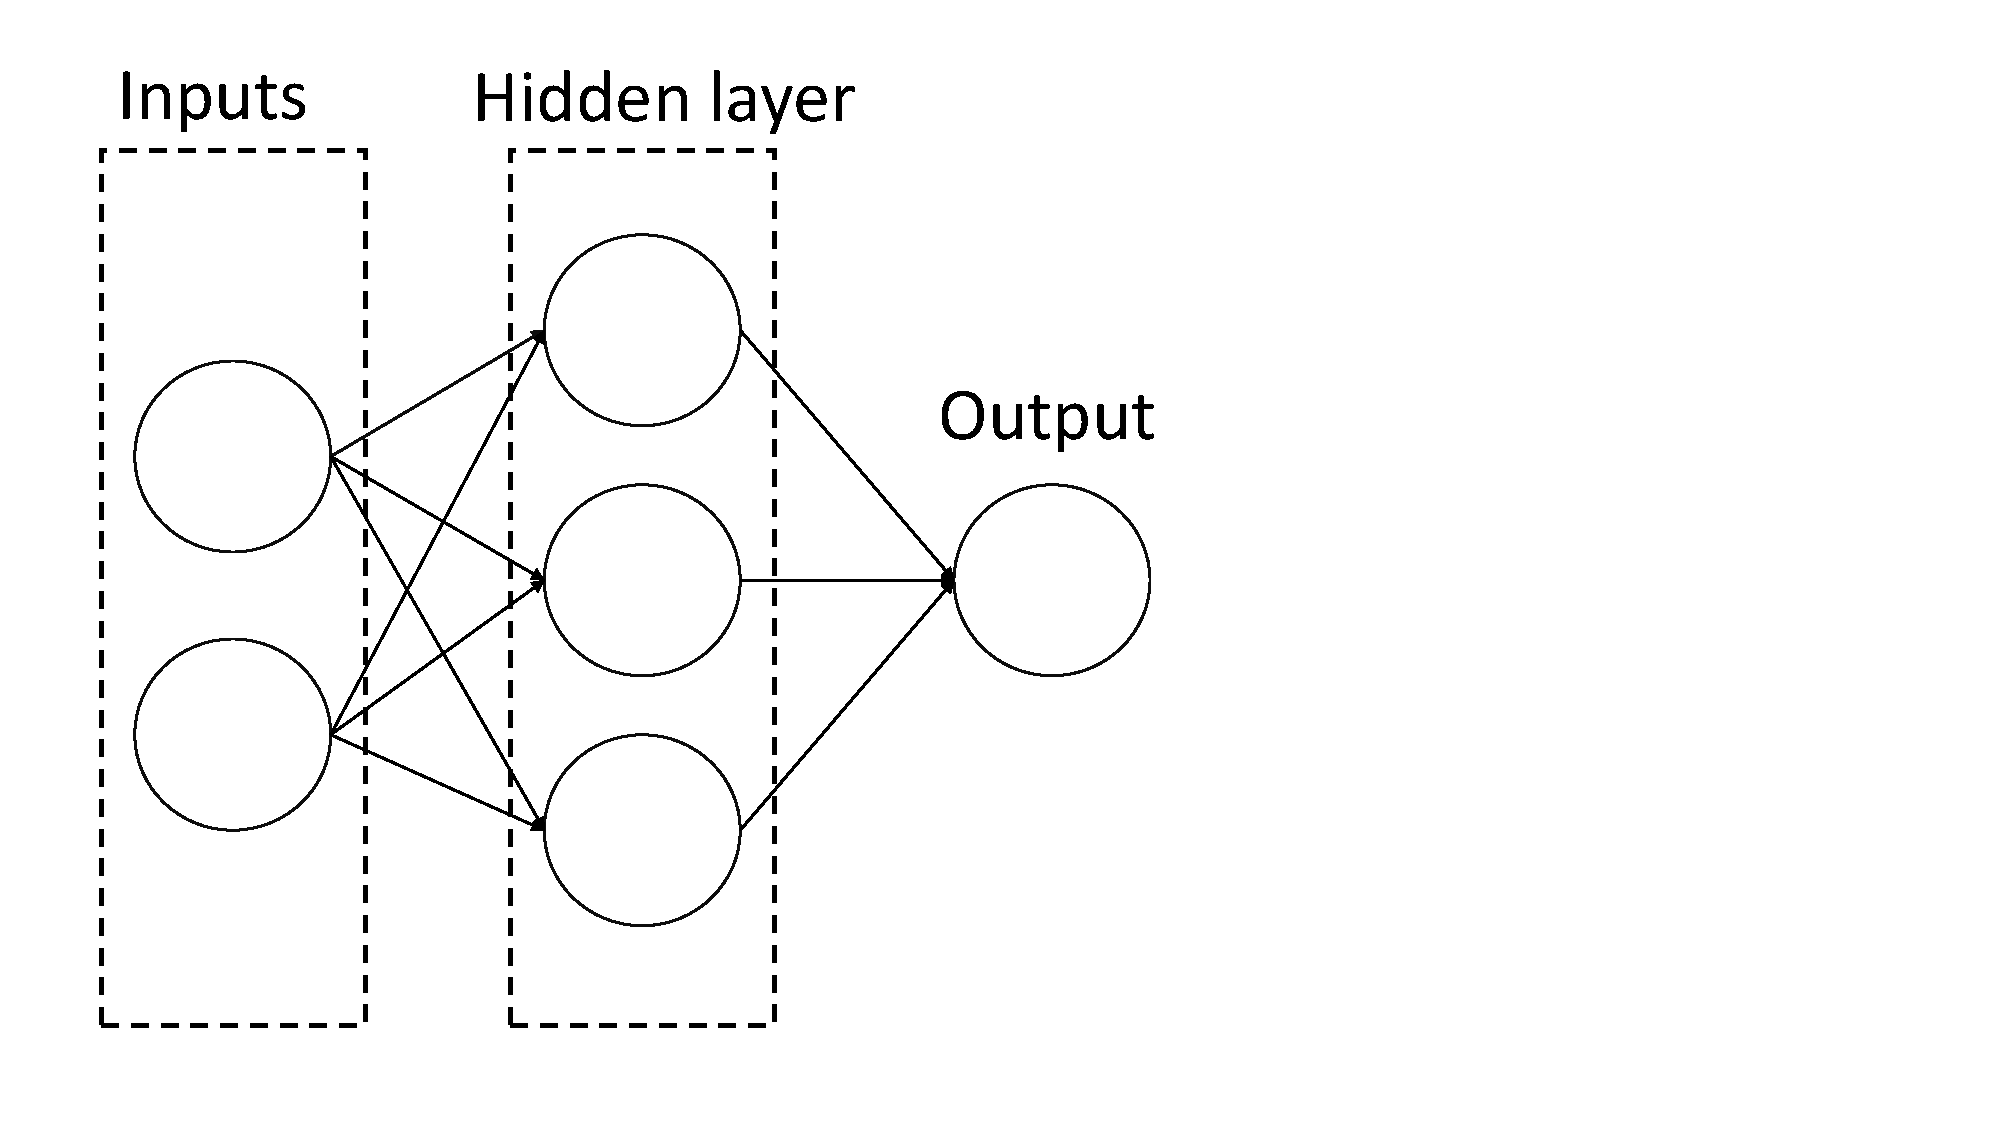
\includegraphics[scale=0.2, trim = 0 0 360 0, clip]{simple_nn/nn_architecture.pdf}
    \caption{Architecture for our simple neural network.}
     \label{fig:nn_arc}
\end{figure}

Denote the two features $x_1$ and $x_2$, the three neurons in the hidden layer $h_1, h_2$, and $h_3$, and the output neuron as $o$. Let the weight from $x_i$ to $h_j$ be $w_{i, j}^{[1]}$ for $i \in \{1, 2\}, j \in \{1, 2, 3\}$, and the weight from $h_j$ to $o$ be $w_{j}^{[2]}$. Finally, denote the intercept weight for $h_j$ as $w_{0, j}^{[1]}$, and the intercept weight for $o$ as $w_{0}^{[2]}$. For the loss function, we'll use average squared loss instead of the usual negative log-likelihood:
$$l = \frac{1}{\nexp}\sum_{i=1}^{\nexp} \left(o^{(i)} - \ysi\right)^2,$$
where $o^{(i)}$ is the result of the output neuron for example $i$.

\begin{enumerate}
  \item \subquestionpoints{5}
Suppose we use the sigmoid function as the activation function for $h_1, h_2, h_3$ and $o$.
What is the gradient descent update to $w_{1, 2}^{[1]}$, assuming we use a learning rate of $\alpha$?
Your answer should be written in terms of $\xsi$, $o^{(i)}$, $\ysi$, and the weights.



\ifnum\solutions=1 {
  \begin{answer}
\end{answer}

} \fi

  \item \subquestionpoints{10} Now, suppose instead of using the sigmoid function for the activation function for $h_1, h_2, h_3$ and $o$, we instead used the step function $f(x)$, defined as
\begin{align*}
f(x) = \begin{cases}
    1, x > 0 \\
    0, x \le 0
    \end{cases}
\end{align*}

Is it possible to have a set of weights that allow the neural network to classify this dataset with 100\% accuracy?

If you believe it's possible, please implement your approach by completing the \texttt{optimal\_step\_weights} method in \texttt{src/simple\_nn/simple\_nn.py} and including the corresponding \texttt{step\_weights.pdf}  plot showing perfect prediction in your writeup.

If it is not possible, please explain your reasoning in the writeup.

\textbf{Hint 1:} There are three sides to a triangle, and there are three neurons in the hidden layer.

\textbf{Hint 2:} A solution can be found where all weight and bias parameters take values only in $\{-1, -0.5, 0, 1, 3, 4 \}$. You are free to come up with other solutions as well.



\ifnum\solutions=1 {
  \begin{answer}
\end{answer}

} \fi

  \item \subquestionpoints{10} Let the activation functions for $h_1, h_2, h_3$ be the linear function $f(x) = x$ and the activation function for $o$ be the same step function as before.

Is it possible to have a set of weights that allow the neural network to classify this dataset with 100\% accuracy?

If you believe it's possible, please implement your approach by completing the \texttt{optimal\_linear\_weights} method in \texttt{src/simple\_nn/simple\_nn.py} and including the corresponding \texttt{linear\_weights.pdf} plot showing perfect prediction in your writeup.

If it is not possible, please explain your reasoning in the writeup.

\textbf{Hint:} The hints from the previous sub-question might or might not apply.


\ifnum\solutions=1 {
  \begin{answer}
\end{answer}

} \fi


\end{enumerate}
